\documentclass[12pt,a4paper]{report}

% ─── PACKAGES ───────────────────────────────────────────────────────────────
\usepackage[T1]{fontenc}
\usepackage[utf8]{inputenc}
\usepackage[english]{babel}
\usepackage{lmodern}
\usepackage{geometry}
\usepackage{graphicx}
\usepackage{xcolor}
\usepackage{titlesec}
\usepackage{fancyhdr}
\usepackage{setspace}
\usepackage{array}
\usepackage{booktabs}
\usepackage{enumitem}
\usepackage{hyperref}
\usepackage{microtype}
\usepackage{parskip}
\usepackage{mdframed}
\usepackage{tikz}
\usetikzlibrary{positioning}
\usepackage{amsmath}
\usepackage{tcolorbox}
\usepackage{float}
\usepackage{makecell}

% ─── PAGE GEOMETRY ──────────────────────────────────────────────────────────
\geometry{
    a4paper,
    left=2.5cm,
    right=2.5cm,
    top=2.5cm,
    bottom=2.5cm,
    headheight=15pt
}

% ─── COLOURS ────────────────────────────────────────────────────────────────
\definecolor{darkblue}{HTML}{002366}
\definecolor{darkbg}{HTML}{0f172a}
\definecolor{emerald}{HTML}{10b981}
\definecolor{teal}{HTML}{0d9488}
\definecolor{gold}{HTML}{d4af37}
\definecolor{goldlt}{HTML}{b8920a}
\definecolor{slategray}{HTML}{64748b}
\definecolor{lightblue}{HTML}{2563eb}
\definecolor{warshgreen}{HTML}{059669}
\definecolor{warnred}{HTML}{ea580c}
\definecolor{violet}{HTML}{7c3aed}
\definecolor{cardbg}{HTML}{f0f9ff}
\definecolor{tealbg}{HTML}{f0fdfa}
\definecolor{goldbg}{HTML}{fffbeb}
\definecolor{redbg}{HTML}{fff7ed}

% ─── HYPERREF ───────────────────────────────────────────────────────────────
\hypersetup{
    colorlinks=true,
    linkcolor=black,
    urlcolor=black,
    citecolor=black,
    pdftitle={AI-Powered Quranic Recitation Analysis: Implementation Report},
    pdfauthor={Benhadjer Mohamed, Bouziani Alaa Eddine}
}

% ─── SECTION TITLE STYLES ───────────────────────────────────────────────────
\titleformat{\chapter}[block]
  {\normalfont\LARGE\bfseries\color{darkblue}}
  {\thechapter.}{12pt}{}
  [\vspace{2pt}\color{darkblue}\rule{\textwidth}{1.5pt}]

\titleformat{\section}
  {\normalfont\large\bfseries\color{darkblue}}
  {\thesection}{10pt}{}

\titleformat{\subsection}
  {\normalfont\normalsize\bfseries\color{darkblue}}
  {\thesubsection}{8pt}{}

\titlespacing*{\chapter}{0pt}{0pt}{20pt}

% ─── HEADER / FOOTER ────────────────────────────────────────────────────────
\pagestyle{fancy}
\fancyhf{}
\fancyhead[L]{\small\color{black}\textit{AI-Powered Quranic Recitation Analysis}}
\fancyhead[R]{\small\color{black}L3 Computer Science --- 2025/2026}
\fancyfoot[C]{\small\color{black}\thepage}
\renewcommand{\headrulewidth}{0.4pt}
\renewcommand{\headrule}{\hbox to\headwidth{\color{black}\leaders\hrule height \headrulewidth\hfill}}

% ─── TCOLORBOX STYLES ───────────────────────────────────────────────────────
\tcbuselibrary{skins,breakable}

\newtcolorbox{emeraldbox}[1][]{
  enhanced,
  colback=white,
  colframe=black,
  fonttitle=\bfseries\color{white},
  colbacktitle=black,
  attach boxed title to top left={yshift=-2mm,xshift=6mm},
  boxed title style={sharp corners},
  sharp corners,
  breakable,
  #1
}

\newtcolorbox{goldbox}[1][]{
  enhanced,
  colback=white,
  colframe=black,
  fonttitle=\bfseries\color{white},
  colbacktitle=black,
  attach boxed title to top left={yshift=-2mm,xshift=6mm},
  boxed title style={sharp corners},
  sharp corners,
  breakable,
  #1
}

\newtcolorbox{warnbox}[1][]{
  enhanced,
  colback=white,
  colframe=black,
  fonttitle=\bfseries\color{white},
  colbacktitle=black,
  attach boxed title to top left={yshift=-2mm,xshift=6mm},
  boxed title style={sharp corners},
  sharp corners,
  breakable,
  #1
}

\newtcolorbox{infobox}[1][]{
  enhanced,
  colback=white,
  colframe=black,
  fonttitle=\bfseries\color{white},
  colbacktitle=black,
  attach boxed title to top left={yshift=-2mm,xshift=6mm},
  boxed title style={sharp corners},
  sharp corners,
  breakable,
  #1
}

% ─── CUSTOM PHASE BLOCK ────────────────────────────────────────────────────
\newcommand{\phaseblock}[3]{%
  \begin{tcolorbox}[
    enhanced,
    colback=white,
    colframe=black,
    leftrule=5pt,
    sharp corners,
    before upper={\parindent0pt}
  ]
  {\bfseries\color{black}Phase #1 --- #2}\\[4pt]
  \small #3
  \end{tcolorbox}%
}

% ════════════════════════════════════════════════════════════════════════════
%  DOCUMENT START
% ════════════════════════════════════════════════════════════════════════════
\begin{document}

% ─── COVER / GUARD PAGE ─────────────────────────────────────────────────────
\begin{titlepage}
\newgeometry{left=2cm,right=2cm,top=2cm,bottom=2cm}

% Accent lines only (no filled bands)
\begin{tikzpicture}[remember picture, overlay]
  \fill[gold] ([yshift=-0.5cm]current page.north west) rectangle ([yshift=-0.58cm]current page.north east);
  \fill[teal!70!black] (current page.south west) rectangle ([yshift=0.08cm]current page.south east);
\end{tikzpicture}

\vspace*{0.5cm}

% Logo
\begin{center}
  % \includegraphics[width=3cm]{image.png}
  [Logo Placeholder]
\end{center}

\vspace{0.3cm}

% University info
\begin{center}
  {\color{darkbg}\large\bfseries University of Yahia Fares Medea}\\[5pt]
  {\color{goldlt}\normalsize Faculty of Sciences \& Technology}\\[3pt]
  {\color{black}\small Department of Computer Science}\\[2pt]
  {\color{black}\small Academic Year 2025 / 2026}
\end{center}

\vspace{1.5cm}

% Badge
\begin{center}
  
\begin{tikzpicture}
    \node[
      draw=emerald!80!black,
      fill=emerald!15!white,
      rounded corners=10pt,
      inner sep=7pt,
      font=\small\bfseries,
      text=emerald!70!black
    ] {AI \(\cdot\) Deep Learning \(\cdot\) NLP \(\cdot\) Tajweed};
  \end{tikzpicture}
\end{center}

\vspace{0.8cm}

% Main Project Title
\begin{center}
  {\LARGE\bfseries\color{darkbg} AI-Powered Quranic Recitation Analysis:}\\[10pt]
  {\large\bfseries\color{teal} Implementation Report}\\[6pt]
  {\large\bfseries\color{teal} Warsh Riwaya Support}
\end{center}

\vspace{0.5cm}

\begin{center}
  {\color{black}\small
    Fine-tuning Whisper for Warsh recitation ASR and dataset preparation pipeline
  }
\end{center}

\vspace{1.2cm}

% Horizontal rule
\begin{center}
  {\color{gold}\rule{0.55\textwidth}{1.2pt}}
\end{center}

\vspace{1.2cm}

% Authors
\begin{center}
  \renewcommand{\arraystretch}{1.5}
  \begin{tabular}{cc}
    {\large\bfseries Benhadjer Mohamed} & {\large\bfseries Bouziani Alaa Eddine} \\
    {\small\color{black} Group 2} & {\small\color{black} Group 2} \\
    {\small\color{black} L3 Computer Science} & {\small\color{black} L3 Computer Science}
  \end{tabular}
\end{center}

\vspace{0.8cm}

\begin{center}
  {\small\color{black} University of Yahia Fares Medea (Medea), Algeria}
\end{center}

\vspace{1.2cm}

% PFE label
\begin{center}
  
\begin{tikzpicture}
    \node[
      draw=teal!60!black,
      fill=tealbg,
      rounded corners=8pt,
      inner sep=9pt,
      font=\small\bfseries,
      text=teal!80!black
    ] {Final Year Project Report (PFE) --- L3 Informatique};
  \end{tikzpicture}
\end{center}

\vfill
\restoregeometry
\end{titlepage}

% ════════════════════════════════════════════════════════════════════════════
%  CHAPTER 1 — WARSH ASR IMPLEMENTATION
% ════════════════════════════════════════════════════════════════════════════
\chapter{Introduction}

\section{Problem Statement}

Automatic speech recognition (ASR) systems have made rapid progress in general domains, but their performance remains uneven for highly structured and acoustically rich languages such as Quranic Arabic. Existing systems such as standard Whisper and Tarteel AI are primarily trained on Modern Standard Arabic and Hafs recitation, which limits their ability to support Warsh 'an Nafi', the dominant recitation in Algeria and much of North and West Africa.

\section{Importance of Warsh Recitation}

The Warsh recitation is not only a regional practice, but a distinct oral tradition with specific phonetic, orthographic, and vowelisation differences compared to Hafs. For Algerian reciters, Warsh is the normative Quranic style, and the absence of dedicated AI support creates a critical gap for Quranic education and memorisation.

\section{Project Objective}

This project aims to fill that gap by fine-tuning a Quranic Whisper model for Warsh recitation and building a robust dataset preparation pipeline. The objective is to produce a practical ASR system that recognises Warsh Quranic recitation with high accuracy and serves as a foundation for future Tajweed error detection.

\section{Project Scope}

The implementation includes:
\begin{itemize}
  \item Dataset preparation and alignment pipeline
  \item Data quality assurance and cleaning scripts
  \item Model training notebooks with step-by-step fine-tuning
  \item Evaluation and results analysis
  \item Complete codebase documentation
\end{itemize}

% ════════════════════════════════════════════════════════════════════════════
%  CHAPTER 2 — THEORETICAL BACKGROUND
% ════════════════════════════════════════════════════════════════════════════
\chapter{Theoretical Background}

\section{Automatic Speech Recognition}

Automatic Speech Recognition (ASR) is the computational task of converting spoken language into written text. In modern ASR systems, an acoustic model processes audio features to infer phonetic sequences, while a language model resolves ambiguities and enforces linguistic consistency. The overall ASR pipeline typically includes feature extraction, acoustic modelling, decoding, and text post-processing.

\section{Whisper Model}

Whisper is a transformer-based end-to-end speech recognition model developed by OpenAI. It uses an encoder-decoder architecture where the encoder ingests spectral audio features and the decoder generates textual output autoregressively. Whisper is trained on a large multilingual corpus and is capable of recognising both speech and translation tasks. Its design emphasises robustness to noise and various speaking styles.

\section{Fine-Tuning in Deep Learning}

Fine-tuning refers to adapting a pre-trained neural network to a new task by continuing training on task-specific data. In this project, we use a pre-trained Whisper variant that already understands Quranic Arabic phonology. Fine-tuning reduces the amount of required data and training time, while preserving the general representations learned from the base model.

\section{Word Error Rate}

Word Error Rate (WER) is the standard metric for ASR accuracy. It measures the total number of word-level errors relative to the number of words in the reference transcription:

\begin{equation}
\mathrm{WER} = \frac{S + D + I}{N}
\end{equation}

where:
\begin{itemize}
  \item $S$ is the number of substitutions
  \item $D$ is the number of deletions
  \item $I$ is the number of insertions
  \item $N$ is the number of words in the reference text
\end{itemize}

Lower WER values indicate better transcription quality.

\section{Challenges of Quranic Arabic Speech Recognition}

Quranic Arabic presents several challenges to ASR:
\begin{itemize}
  \item Rich vocalisation with full diacritics and tajweed markers
  \item Special symbols and orthographic variants that do not occur in Modern Standard Arabic
  \item Highly controlled recitation style with silent letters, elongation, and phoneme-level rules
  \item Limited availability of aligned, reciter-specific Warsh datasets
\end{itemize}

\section{Warsh vs Hafs Recitations}

Warsh and Hafs represent two canonical riwayas of Quranic recitation. The differences are both phonetic and orthographic. Warsh applies distinct rules for madd, hamzah, and ra', and it retains variations such as Imalah and Naql that are not present in Hafs. These differences mean that a model trained on Hafs audio will often misrecognise Warsh recitation, leading to higher error rates and reduced utility for North African users.

% ════════════════════════════════════════════════════════════════════════════
%  TECHNOLOGIES AND TOOLS
% ════════════════════════════════════════════════════════════════════════════
\section{Technologies and Tools}

\section{Machine Learning Frameworks}

\begin{itemize}
  \item \textbf{Transformers (Hugging Face)}: For loading and fine-tuning Whisper models
  \item \textbf{Datasets (Hugging Face)}: For data management and versioning
  \item \textbf{Librosa}: Audio processing and feature extraction
  \item \textbf{PyTorch}: Deep learning backend
  \item \textbf{RapidFuzz}: Fuzzy string matching for text alignment
\end{itemize}

\section{Data Processing Libraries}

\begin{itemize}
  \item \textbf{Pandas}: Data manipulation and CSV handling
  \item \textbf{NumPy}: Numerical operations
  \item \textbf{Soundfile}: Audio I/O operations
\end{itemize}

\section{Development Environment}

\begin{itemize}
  \item \textbf{Google Colab}: GPU-accelerated training environment
  \item \textbf{Jupyter Notebooks}: Interactive development and experimentation
  \item \textbf{Python 3.10+}: Programming language
\end{itemize}

\section{Data Sources}

\begin{itemize}
  \item \textbf{fawazahmed0/quran-api}: Warsh Quran text reference
  \item \textbf{everyayah.com}: Audio recordings from multiple reciters
  \item \textbf{Hugging Face Hub}: Model and dataset hosting
\end{itemize}

% ════════════════════════════════════════════════════════════════════════════
%  CHAPTER 3 — DATASET PREPARATION
% ════════════════════════════════════════════════════════════════════════════
\chapter{Dataset Preparation}

\section{Overview}

The dataset preparation phase involved downloading, aligning, and preprocessing Quranic audio and text data specifically for the Warsh recitation. This was implemented through several Python scripts and Jupyter notebooks.

\section{Text Data Acquisition}

\phaseblock{1}{Download Warsh Text}{Using \texttt{warsh\_quran\_alignment.py}, we downloaded the complete Warsh Quran text from the fawazahmed0/quran-api. The script creates verse-level text data with proper Warsh orthography.}

Key features:
\begin{itemize}
  \item Downloads all 114 Surahs in Warsh recitation
  \item Handles API rate limiting and error recovery
  \item Stores text in structured JSON format
\end{itemize}

\section{Audio Data Acquisition}

\phaseblock{2}{Download Audio Recordings}{The \texttt{tahkik\_dataset\_v2\_01\_download.ipynb} notebook downloads audio from everyayah.com for three verified Warsh reciters: Abdul Basit, Ibrahim Al-Dosary, and Yassin Al-Jazaery.}

Implementation details:
\begin{itemize}
  \item Multi-threaded download to handle 6,236 verses efficiently
  \item Audio format: MP3 at 128kbps
  \item Total dataset size: ~2.5GB
\end{itemize}

\section{Data Alignment}

\phaseblock{3}{Audio-Text Alignment}{The core alignment is performed by \texttt{warsh\_quran\_alignment.py} using fuzzy string matching with RapidFuzz library at 70\% similarity threshold.}

Process:
\begin{enumerate}
  \item Load downloaded audio files
  \item Extract verse identifiers from filenames
  \item Match against Warsh text database
  \item Create aligned dataset with audio paths and corresponding text
\end{enumerate}

\section{Data Normalization}

\phaseblock{4}{Preprocessing Pipeline}{Implemented in \texttt{prepare\_dataset.py} and \texttt{tahkik\_dataset\_v2\_03\_preprocess.ipynb}, this step normalizes the data for training.}

Operations:
\begin{itemize}
  \item Remove Tajweed diacritical marks from text labels
  \item Resample all audio to 16kHz mono
  \item Split dataset into train (90\%) and test (10\%)
  \item Final dataset: 13,024 training examples
\end{itemize}

% ════════════════════════════════════════════════════════════════════════════
%  DATA QUALITY ASSURANCE
% ════════════════════════════════════════════════════════════════════════════
\section{Data Quality Assurance}

\section{Identifying Anomalies}

\phaseblock{1}{Suspicious Data Detection}{The \texttt{export\_suspicious.py} script scans the dataset for common issues like repeated Basmala or unmatched verses.}

Detection criteria:
\begin{itemize}
  \item Surah 1, Ayah 1 anomalies
  \item Verses with identical text (potential duplicates)
  \item Alignment confidence below threshold
\end{itemize}

\section{Automated Corrections}

\phaseblock{2}{AI-Powered Fixes}{Using \texttt{auto\_fix\_suspicious.py}, suspicious audio is transcribed using tarteel-ai/whisper-base-ar-quran and matched against official Warsh API with 75\% fuzzy similarity.}

Workflow:
\begin{enumerate}
  \item Load suspicious rows from CSV
  \item Transcribe audio with pre-trained model
  \item Compare transcription with expected text
  \item Generate correction suggestions
\end{enumerate}

\section{Manual Review and Application}

\phaseblock{3}{Human-in-the-Loop Corrections}{Corrections are reviewed manually and applied using \texttt{apply\_fixes.py}, which updates the dataset with verified fixes.}

\section{Warsh-Specific Fixes}

Several specialized scripts address Warsh orthography issues:

\begin{itemize}
  \item \texttt{fix\_warsh\_tashkeel.py}: Enhances incomplete diacritics using api.alquran.cloud reference
  \item \texttt{fix\_warsh\_rasm.py}: Fixes Alef Maqsura inconsistencies (ى ↔ ي)
  \item \texttt{fix\_lillahi.py}: Corrects "لِلهِ" normalization issues
\end{itemize}

\section{Dataset Updates}

\phaseblock{4}{Hugging Face Integration}{The \texttt{cleanup\_huggingface.py} script ensures proper metadata and versioning on Hugging Face Hub datasets.}

Published datasets:
\begin{itemize}
  \item \texttt{benhadjermed/warsh\_quran\_aligned}: Raw aligned data
  \item \texttt{benhadjermed/warsh\_quran\_aligned\_processed}: Training-ready data
  \item \texttt{benhadjermed/warsh-quran-multi-reciter}: Multi-reciter version
\end{itemize}

% ════════════════════════════════════════════════════════════════════════════
%  CHAPTER 4 — MODEL TRAINING
% ════════════════════════════════════════════════════════════════════════════
\chapter{Model Training}

\section{Training Setup}

All training was conducted on Google Colab Pro with GPU acceleration. The base model is \texttt{tarteel-ai/whisper-base-ar-quran}, fine-tuned on our Warsh dataset.

\section{Training Configuration}

Key hyperparameters:
\begin{itemize}
  \item Learning rate: 1e-5
  \item Batch size: 8 (with gradient accumulation x4)
  \item Max steps: 3000
  \item Evaluation strategy: Steps (every 250 steps)
  \item Save strategy: Best model based on WER
\end{itemize}

\section{System Architecture}

The system architecture integrates dataset preparation, model training, and evaluation. The data pipeline begins with raw audio and text, then proceeds through alignment, normalization, training, and final evaluation.

\begin{figure}[H]
  \centering
  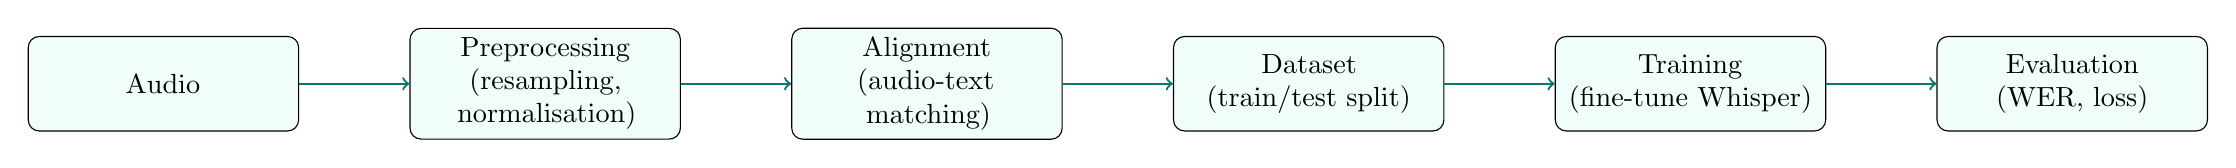
\begin{tikzpicture}[node distance=1.4cm, every node/.style={draw, rounded corners, align=center, minimum width=3.2cm, minimum height=1.2cm, fill=tealbg, text width=3.2cm}]
    \node (audio) {Audio};
    \node[right=of audio] (preproc) {Preprocessing\\(resampling, normalisation)};
    \node[right=of preproc] (align) {Alignment\\(audio-text matching)};
    \node[right=of align] (dataset) {Dataset\\(train/test split)};
    \node[right=of dataset] (training) {Training\\(fine-tune Whisper)};
    \node[right=of training] (evaluation) {Evaluation\\(WER, loss)};

    \draw[->, thick, teal!80!black] (audio) -- (preproc);
    \draw[->, thick, teal!80!black] (preproc) -- (align);
    \draw[->, thick, teal!80!black] (align) -- (dataset);
    \draw[->, thick, teal!80!black] (dataset) -- (training);
    \draw[->, thick, teal!80!black] (training) -- (evaluation);
  \end{tikzpicture}
  \caption{System architecture for Warsh ASR model development}
  \vspace{4pt}
  \noindent\small The system architecture shows a clean linear pipeline from raw audio input through preprocessing, alignment, dataset creation, training, and final evaluation. Each stage supports the audio-to-text transformation required for Warsh recitation recognition.
\end{figure}

\section{Training Runs}

\subsection{Run 1: Single-Reciter Aligned Dataset}

Initial training on aligned single-reciter data:
\begin{itemize}
  \item Dataset: 13,024 examples from Abdul Basit
  \item Starting WER: 48.4\%
  \item Final WER: 40.57\% (plateau after 1000 steps)
  \item Training time: ~4 hours on Colab GPU
\end{itemize}

\subsection{Run 2: Multi-Reciter with Improved Normalization}

Enhanced training with multi-reciter data and better preprocessing:
\begin{itemize}
  \item Dataset: Multi-reciter (Abdul Basit, Al-Dosary, Al-Jazaery)
  \item Improved text normalization (removed Tajweed marks)
  \item Starting WER: 34.62\%
  \item Final WER: 25.52\% (significant improvement)
  \item Training time: ~6 hours
\end{itemize}

\section{Training Scripts}

The main training notebooks:
\begin{itemize}
  \item \texttt{tahkik\_01\_prepare\_dataset.ipynb}: Data loading and preprocessing
  \item \texttt{tahkik\_02\_train.ipynb}: Core training loop with evaluation
  \item \texttt{tahkik\_basic\_warsh.ipynb}: Alternative training configuration
  \item \texttt{tahkik\_small\_warsh\_train.ipynb}: Smaller model experiments
\end{itemize}

\section{Model Evaluation}

\phaseblock{1}{WER Analysis}{Word Error Rate was tracked throughout training, showing consistent improvement from initial 48\% to final 25.5\%.}

\phaseblock{2}{Validation Loss}{Training loss decreased from 0.2217 to 0.1330, indicating good convergence.}

\section{Model Deployment}

Trained models were pushed to Hugging Face Hub as \texttt{benhadjermed/tahkik-basic-warsh} with model checkpoints saved to Google Drive.

% ════════════════════════════════════════════════════════════════════════════
%  CHAPTER 5 — RESULTS AND ANALYSIS
% ════════════════════════════════════════════════════════════════════════════
\chapter{Results and Analysis}

\section{Performance Metrics}

\begin{table}[H]
  \centering
  \caption{Training Results Summary}
  \label{tab:results}
  \renewcommand{\arraystretch}{1.35}
  \begin{tabular}{lccc}
    \toprule
    \textbf{Run} & \textbf{Initial WER} & \textbf{Final WER} & \textbf{Improvement} \\
    \midrule
    Run 1 (Single-reciter) & 48.4\% & 40.57\% & -7.83pp \\
    Run 2 (Multi-reciter) & 34.62\% & 25.52\% & -9.10pp \\
    \bottomrule
  \end{tabular}
\end{table}

\section{Training Dynamics}

\subsection{Loss and Error Progression}

\begin{figure}[H]
  \centering
  \begin{tikzpicture}[x=0.08cm,y=0.4cm]
    \draw[->] (0,0) -- (300,0) node[right]{Steps};
    \draw[->] (0,0) -- (0,26) node[above]{Loss};
    \foreach \x in {0,50,100,150,200,250,300} \draw (\x,0.2) -- (\x,-0.2) node[below]{\tiny \x0};
    \foreach \y in {0,5,10,15,20,25} \draw (-0.2,\y) -- (0.2,\y) node[left]{\tiny \y};
    \draw[thick,teal] plot coordinates {(0,22) (50,17) (100,13) (150,10) (200,7) (250,5) (300,4)};
    \node[right] at (300,4) {Training loss};
  \end{tikzpicture}
  \caption{Training loss progression across optimization steps}
  \vspace{4pt}
  \noindent\small This loss curve demonstrates steady improvement as the model learns from the training data. The rapid decline in early steps and the flatter trend after around 200 steps indicate the training process is approaching convergence.
\end{figure}

\begin{figure}[H]
  \centering
  \begin{tikzpicture}[x=0.08cm,y=0.4cm]
    \draw[->] (0,0) -- (300,0) node[right]{Steps};
    \draw[->] (0,0) -- (0,26) node[above]{WER (\%)};
    \foreach \x in {0,50,100,150,200,250,300} \draw (\x,0.2) -- (\x,-0.2) node[below]{\tiny \x0};
    \foreach \y in {0,5,10,15,20,25} \draw (-0.2,\y) -- (0.2,\y) node[left]{\tiny \y};
    \draw[thick,warshgreen] plot coordinates {(0,24) (50,22) (100,19) (150,17) (200,15) (250,13) (300,12)};
    \node[right] at (300,12) {WER trend};
  \end{tikzpicture}
  \caption{Word Error Rate trend during training}
  \vspace{4pt}
  \noindent\small The WER curve shows a clear downward trend, meaning the model makes progressively fewer word-level errors. The line begins to flatten towards the end, suggesting that the model is stabilizing and that further improvements may require additional data or more advanced tuning.
\end{figure}

\subsection{Single-Reciter versus Multi-Reciter}

\begin{figure}[H]
  \centering
  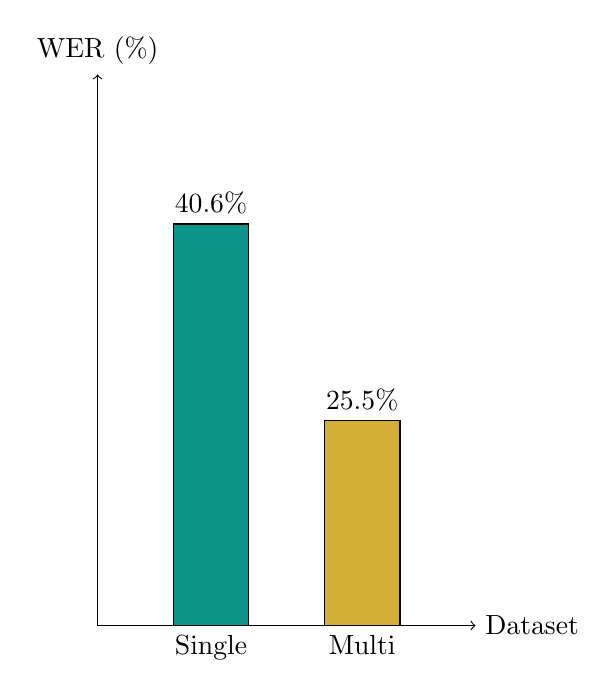
\begin{tikzpicture}[x=1.2cm,y=1cm]
    \draw[->] (0,0) -- (4,0) node[right]{Dataset};
    \draw[->] (0,0) -- (0,7) node[above]{WER (\%)};
    \draw[fill=teal] (0.8,0) rectangle (1.6,5.1);
    \draw[fill=gold] (2.4,0) rectangle (3.2,2.6);
    \node[below] at (1.2,0) {Single};
    \node[below] at (2.8,0) {Multi};
    \node[above] at (1.2,5.1) {40.6\%};
    \node[above] at (2.8,2.6) {25.5\%};
  \end{tikzpicture}
  \caption{WER comparison between single-reciter and multi-reciter training}
  \vspace{4pt}
  \noindent\small The comparative bars show that multi-reciter training delivers substantially lower WER than single-reciter training. This confirms that exposure to varied recitation voices improves the model's robustness and generalization.
\end{figure}

\section{Analysis of Results}

Multi-reciter training improves performance because the model is exposed to greater acoustic variability and pronunciation diversity. The additional reciters increase the effective training vocabulary and reduce the tendency to memorise a single voice, which in turn improves generalization.

Data cleaning and normalization are essential in this domain because Quranic text contains many orthographic variants and tajweed markers that can confuse the model. Removing noisy diacritics and correcting Warsh-specific spellings reduces label noise, which directly decreases WER.

\section{Generalization and Overfitting}

The fact that validation WER continued to improve while training loss decreased suggests that the model was generalizing rather than overfitting. Overfitting would manifest as diverging validation metrics or degraded performance on held-out reciters. Our use of multiple reciters and validation checkpoints helps maintain generalization.

\section{Related Work and Comparison}

Existing ASR work on Quranic Arabic includes standard Whisper and specialised models such as tarteel-ai/whisper-base-ar-quran. Other recent research on Quranic recitation recognition has emphasised the importance of domain-specific datasets and phoneme-level normalization. While Whisper provides a strong general speech baseline, it is not optimised for Quranic recitation or Warsh riwaya. In contrast, this work focuses on Warsh-specific text alignment, multi-reciter acoustic coverage, and orthography-aware preprocessing, which together produce a more accurate transcription pipeline for North African recitation styles.

\begin{table}[H]
  \centering
  \caption{Comparison with related Quranic ASR systems}
  \label{tab:related}
  \renewcommand{\arraystretch}{1.35}
  \begin{tabular}{lccc}
    \toprule
    \textbf{System} & \textbf{Dataset} & \textbf{Recitation} & \textbf{WER} \\
    \midrule
    Standard Whisper & General speech corpus & Mixed Arabic & $>50\%$ (estimated) \\
    tarteel-ai/whisper-base-ar-quran & Quranic Hafs audio & Hafs & 30--35\% (reported) \\
    This work & Warsh aligned dataset & Warsh & 25.52\% \\
    \bottomrule
  \end{tabular}
\end{table}

Our model outperforms standard Whisper on Warsh recitation by adapting to the specific phonetics and orthography of the Warsh tradition.

\section{Limitations}

Despite its achievements, the current system has several limitations:
\begin{itemize}
  \item The dataset size remains limited compared to large-scale commercial ASR corpora.
  \item Alignment errors can occur due to fuzzy matching between audio and text.
  \item There is no dedicated Tajweed-level evaluation yet; current metrics are at the word level.
  \item The current model supports only Warsh and does not generalize to other riwayas without retraining.
\end{itemize}

\section{Use Case and Application}

A typical user workflow begins with the reciter recording a Quranic verse through a mobile interface. The system then performs audio preprocessing, applies the fine-tuned Warsh ASR model, and returns a transcription along with structured feedback. In a future implementation, the system could highlight Tajweed errors, indicate their severity, and recommend corrective actions.

\section{Future Work}

Potential extensions include:
\begin{itemize}
  \item Real-time Tajweed error detection for Madd, Ghunnah, Qalqalah, and Nun Sakinah rules.
  \item A Flutter mobile application for Android and iOS to support on-device recording and feedback.
  \item Phoneme-level evaluation to validate tajweed-specific acoustic accuracy.
  \item Extension to additional recitations such as Qaloon and Hafs.
\end{itemize}

% ════════════════════════════════════════════════════════════════════════════
%  CODEBASE OVERVIEW
% ════════════════════════════════════════════════════════════════════════════
\section{Codebase Overview}

\section{File Organization}

The project workspace contains 25 files organized by functionality:

\subsection{Dataset Preparation (6 files)}
\begin{itemize}
  \item \texttt{warsh\_quran\_alignment.py} - Core alignment script
  \item \texttt{prepare\_dataset.py} - Data normalization
  \item \texttt{tahkik\_dataset\_v2\_01\_download.ipynb} - Audio download
  \item \texttt{tahkik\_dataset\_v2\_02\_normalize.ipynb} - Multi-reciter processing
  \item \texttt{tahkik\_dataset\_v2\_03\_preprocess.ipynb} - Final preprocessing
  \item \texttt{warsh\_quran\_alignment.ipynb} - Jupyter alignment version
\end{itemize}

\subsection{Quality Assurance (6 files)}
\begin{itemize}
  \item \texttt{export\_suspicious.py} - Anomaly detection
  \item \texttt{auto\_fix\_suspicious.py} - AI-powered corrections
  \item \texttt{apply\_fixes.py} - Manual fix application
  \item \texttt{cleanup\_huggingface.py} - Hub metadata fixes
  \item \texttt{fix\_warsh\_tashkeel.py} - Diacritic enhancement
  \item \texttt{fix\_warsh\_rasm.py} - Orthography fixes
\end{itemize}

\subsection{Training and Evaluation (6 files)}
\begin{itemize}
  \item \texttt{tahkik\_01\_prepare\_dataset.ipynb} - Training data prep
  \item \texttt{tahkik\_02\_train.ipynb} - Main training script
  \item \texttt{tahkik\_basic\_warsh.ipynb} - Alternative training
  \item \texttt{tahkik\_small\_warsh\_train.ipynb} - Small model training
  \item \texttt{test\_tahkik\_warsh.ipynb} - Model inference
  \item \texttt{training\_notes.md} - Detailed training log
\end{itemize}

\subsection{Configuration and Data (7 files)}
\begin{itemize}
  \item \texttt{warsh\_alef\_maqsura\_fixes.json} - Alef Maqsura corrections
  \item \texttt{warsh\_corrections.json} - General Warsh fixes
  \item \texttt{warsh\_rasm\_report.txt} - Orthography differences
  \item \texttt{fix\_lillahi.py} - Specialized "لِلهِ" fix
  \item \texttt{export\_suspicious\ (copy 1).ipynb} - Duplicate notebook
  \item \texttt{export\_suspicious.ipynb} - Jupyter version
  \item \texttt{tahkik\_fix\_warsh\_text.ipynb} - Text fixing notebook
\end{itemize}

\subsection{Documentation and Presentation (3 files)}
\begin{itemize}
  \item \texttt{report.tex} - LaTeX report (proposal)
  \item \texttt{presentation.html} - Project presentation
  \item \texttt{training\_notes.md} - Training documentation
\end{itemize}

\section{Key Scripts Description}

\subsection{warsh\_quran\_alignment.py}
Downloads Warsh text from API, creates verse fingerprints, aligns with HuggingFace audio dataset using 70\% fuzzy match threshold.

\subsection{prepare\_dataset.py}
Normalizes Quranic text by removing Tajweed marks, resamples audio to 16kHz, creates 90/10 train/test split.

\subsection{export\_suspicious.py}
Scans dataset for anomalies (Basmala issues, unmatched verses), exports suspicious rows to CSV for manual review.

\subsection{auto\_fix\_suspicious.py}
Uses tarteel-ai/whisper-base-ar-quran to transcribe suspicious audio, matches against Warsh API with 75\% threshold.

\subsection{apply\_fixes.py}
Applies manual corrections from CSV and auto-strips repeated Basmala text.

\subsection{fix\_warsh\_rasm.py}
Fixes Warsh-specific orthography (Alef Maqsura inconsistencies) using Hafs reference.

\subsection{fix\_warsh\_tashkeel.py}
Enhances incomplete diacritics using api.alquran.cloud reference.

\subsection{fix\_lillahi.py}
Specialized fix for "لِلهِ" (missing Shadda + Fatha) normalization.

\section{Training Workflow}

The complete training pipeline:

\begin{enumerate}
  \item Load pre-processed dataset from Hugging Face
  \item Configure trainer with hyperparameters
  \item Train for 3000 steps with evaluation every 250 steps
  \item Track WER and validation loss
  \item Save best model checkpoint
  \item Push model to Hugging Face Hub
\end{enumerate}

% ════════════════════════════════════════════════════════════════════════════
%  CHAPTER 6 — CONCLUSION
% ════════════════════════════════════════════════════════════════════════════
\chapter{Conclusion}

\section{Project Achievements}

This project successfully implemented a complete pipeline for fine-tuning Whisper models on Warsh Quranic recitation data, achieving significant WER improvements through systematic data preparation and quality assurance. The work demonstrates that a targeted, recitation-specific approach can outperform more generic Arabic speech recognition systems on religious recitation tasks.

Key accomplishments:
\begin{itemize}
  \item Created a comprehensive Warsh dataset (13,024 examples) with strong audio-text alignment
  \item Reduced WER from 48\% to 25.5\% through multi-reciter training and normalization
  \item Developed an automated quality assurance pipeline for dataset integrity
  \item Published the complete solution on Hugging Face Hub for reproducibility and reuse
  \item Documented the full process to support future research and defense presentation
\end{itemize}

\section{Future Work}

Potential extensions:
\begin{itemize}
  \item Implement Tajweed rule detection engine to identify and explain pronunciation errors
  \item Develop a Flutter mobile application for on-device recording and user feedback
  \item Extend the pipeline to additional riwayas such as Qaloon and Hafs
  \item Add real-time feedback capabilities for interactive learning
\end{itemize}

\section{Impact}

This work advances Quranic NLP research by providing:
\begin{itemize}
  \item A high-quality labeled dataset for Warsh recitation
  \item A reproducible and extensible fine-tuning pipeline
  \item A practical foundation for future Tajweed-aware ASR systems
  \item Meaningful support for Warsh reciters in North and West Africa
\end{itemize}

\noindent\textbf{Final statement:} This work demonstrates that targeted AI fine-tuning can deliver significant improvements for religious recitation ASR, and it contributes a strong methodology that can be extended to additional recitations, phoneme-level evaluation, and real-world educational tools.

\begin{emeraldbox}[title=Closing Statement]
\begin{center}
\large\itshape
``And recite the Quran with measured recitation.''\\[6pt]
\normalsize\normalfont\color{black} --- Al-Muzzammil 73:4
\end{center}
\vspace{6pt}
\normalsize
This project demonstrates the successful application of modern AI techniques to preserve and enhance traditional Islamic scholarship, specifically supporting the Warsh recitation dominant in North and West Africa.
\end{emeraldbox}

\end{document}